\documentclass[paper=a4, fontsize=11pt]{scrartcl} % A4 paper and 11pt font size
\usepackage{listings}
\usepackage[T1]{fontenc} % Use 8-bit encoding that has 256 glyphs
\usepackage{fourier} % Use the Adobe Utopia font for the document - comment this line to return to the LaTeX default
\usepackage[english]{babel} % English language/hyphenation
\usepackage{amsmath,amsfonts,amsthm} % Math packages
\usepackage{hyperref}
\usepackage{lipsum} % Used for inserting dummy 'Lorem ipsum' text into the template
\usepackage{graphicx}
\usepackage[rightcaption]{sidecap}
\graphicspath{ {fig/} }
\usepackage{booktabs}
\usepackage{skmath}

\ExplSyntaxOn
\RenewDocumentCommand\log{oom}{%
  \IfNoValueTF{#1}
    {\ensuremath{\__skmath_log:\IfNoValueTF{#2}{}{\c_math_superscript_token{#2}}\__skmath_parens:n{#3}}}
    {\ensuremath{\__skmath_log:\c_math_subscript_token{#1}\IfNoValueTF{#2}{}{\c_math_superscript_token{#2}}\__skmath_parens:n{#3}}}%
}
\ExplSyntaxOff

\usepackage{caption}
\usepackage{float}
\usepackage{tabu}
\usepackage{color}
\usepackage{listings}
\usepackage{xcolor}
\usepackage{courier} 
\usepackage{mathrsfs}
\usepackage{sectsty} % Allows customizing section commands
\allsectionsfont{\centering\normalfont \scshape} 
\usepackage{enumitem}
\usepackage{fancyhdr}
\pagestyle{fancy}
\fancyhf{}
\rhead{\textit{TCSS543 Homework 3} }
\lhead{ \textit{Jiacheng Liu, jiachl5@uw.edu} }
\cfoot{Page \thepage}
\numberwithin{equation}{section} % Number equations within sections (i.e. 1.1, 1.2, 2.1, 2.2 instead of 1, 2, 3, 4)
\numberwithin{figure}{section} % Number figures within sections (i.e. 1.1, 1.2, 2.1, 2.2 instead of 1, 2, 3, 4)
\numberwithin{table}{section} % Number tables within sections (i.e. 1.1, 1.2, 2.1, 2.2 instead of 1, 2, 3, 4)

\setlength\parindent{0pt} % Removes all indentation from paragraphs - comment this line for an assignment with lots of text

%----------------------------------------------------------------------------------------
%	TITLE SECTION
%----------------------------------------------------------------------------------------

\newcommand{\horrule}[1]{\rule{\linewidth}{#1}} % Create horizontal rule command with 1 argument of height

\title{	
\normalfont \normalsize 
\textsc{University of Washington} \\ [25pt] % Your university, school and/or department name(s)
\horrule{0.5pt} \\[0.3cm] % Thin top horizontal rule
\huge TCSS 543 Advanced Algorithms \\ % The assignment title
\large \textit{Winter, 2017 Homework 3 }
%\horrule{2pt} \\[0.5cm] % Thick bottom horizontal rule
}

\author{Jiacheng Liu} % Your name

\date{\normalsize\today} % Today's date or a custom date

\begin{document}

\maketitle % Print the title


\section{Problem 1 and 2 }

\subsection{Analysis}
The \textit{DSatur algorithm} colors one node per iteration. So the worst-case time complexity is at least $O(|V|f(|V|,|E|))$. In the inner loop, \textit{Color the chosen vertex with the least possible color} takes at most $O(|V|)$. Imagine an array $A$ of length $|V|$ initialized by value $0$, its index corresponding to the colors which may be used. Since there is at most $|V|$ different colors, we can number them with integers from $0$ to $n-1$. We can choose the least possible color by iterating this array twice. In the first iteration, every node is visited and if it is colored with $i$, then set $A[i]=1$. In the second iteration, we we start from $A[0]$ until we find $A[k] \neq 1 $. Then we can assign color $k$ to this vertex. Therefore, if we can improve the process of choosing the maximal saturation degree vertex, then the problem is solved. 

\subsection{Algorithm}
A maximum heap can be used to improve the worst-case complexity. Both the worst-case complexity and the average time complexity are $O(|V||E|log(|V|))$.  When choosing a vertex, a ``remove" (or ``pop") operation is executed and its complexity is $O(log(|V|))$. To obtain a better constant, in the implemented algorithm, instead of adding all vertex to the max heap at very first, vertices are inserted into the max heap only when one of its neighbor is colored at the first time. Every time a vertex is colored, all its uncolored neighbor are inserted into the max heap. If already in the heap, then a $siftUp$ method is invoked to adjust the heap. Therefore the worst and the average complexity of maintaining a max heap is $O(|E|log(|V|))$ which gives the overall complexity of $O(|V||E|log(|V|))$ .

\newpage

\section{Problem 3}
\subsection{Generating Random Graphs}
Graphs are generated using the methods in the original paper\cite{DSatur}. However, in order to ensure the graph is connected, a slightly different approach is adopted. A random spanning tree is generated in the first step, then a modified density is applied since there are already $n-1$edges chosen. Rest of edges are selected based on the algorithm mentioned in the original paper. If the target density is $d$, let the maximum possible number of edges $t=\frac{|V|(|V|-1)}{2}$, then the modified density is $\frac{td-|V|+1}{t-|V|+1}$.
\subsection{Applying DSatur}
For each combination of density (equals to $0.3, 0.5, 0.65, 0.75$) and number of vertices($10,20, ... 100$), 100 graphs are generated. Then the running time and other statistics are measured. Table \ref{tab:running time (density=0.3)}\ref{tab:running time (density=0.5)}\ref{tab:running time (density=0.65)}\ref{tab:running time (density=0.75)} have detailed results. The data have been divided by 100 to get the average running time on one graph. The unit is $10^{-3}$ seconds. 
\begin{figure}[htp]
\centering
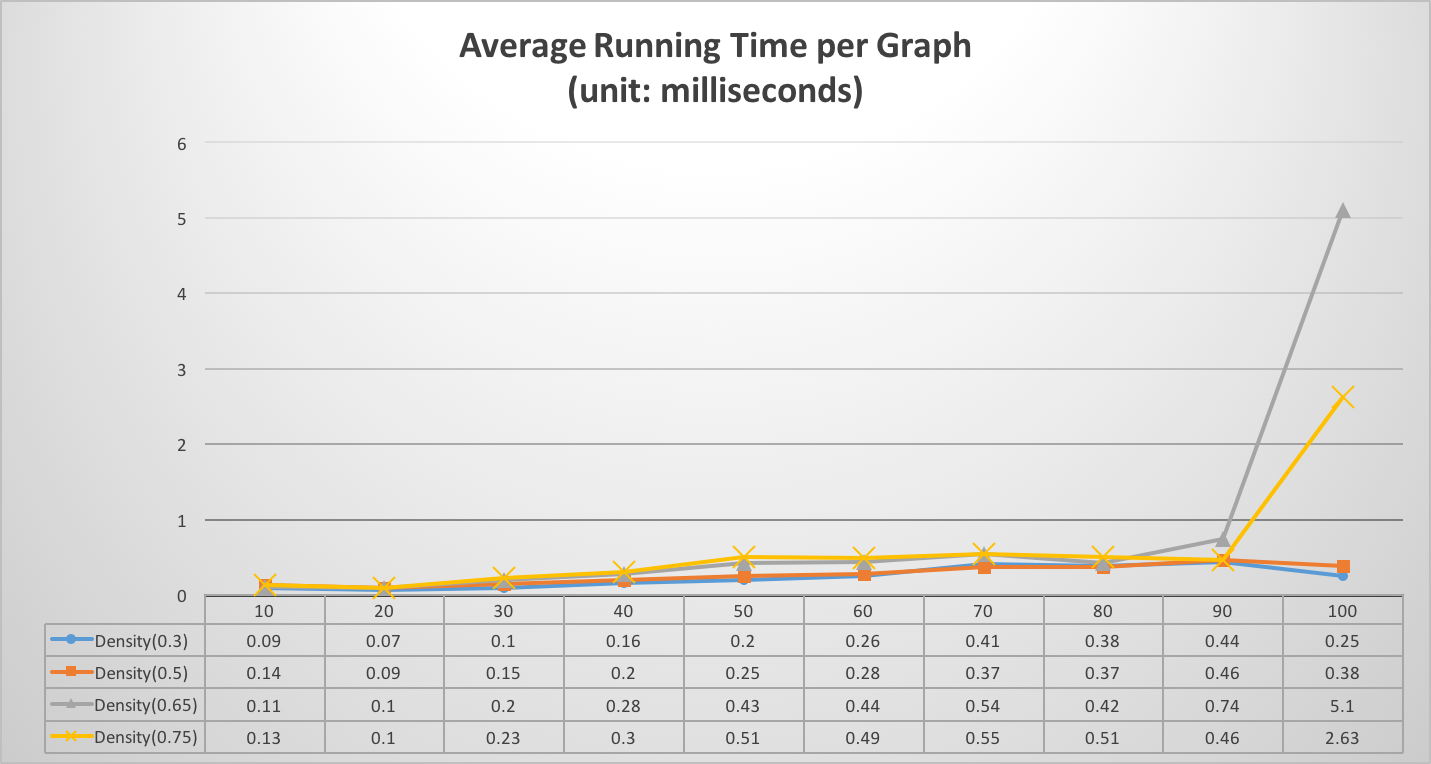
\includegraphics[width=13cm]{runningtime}
\centering
\caption{Running time of implemented DSatur. }
\label{fig:runtime}
\end{figure}

Although non-related programs are turned off before running, there are still unexpected fluctuations in the running time. As Figure\ref{fig:runtime} shows, when density is low ($d = 0.3, 0.5$), the algorithm actually preform better on 100-node graphs then on 90-node graphs.  However, the trend still looks like polynomial, which serves as a confirmation of the analysis in the previous section.

\section{Problem 4}

For more detailed results and data, please refer to section \ref{sec:data}. Figure \ref{fig:mincolor} shows the results of the experiments. This graph comes from the experiments.
\begin{figure}[htp]
\centering
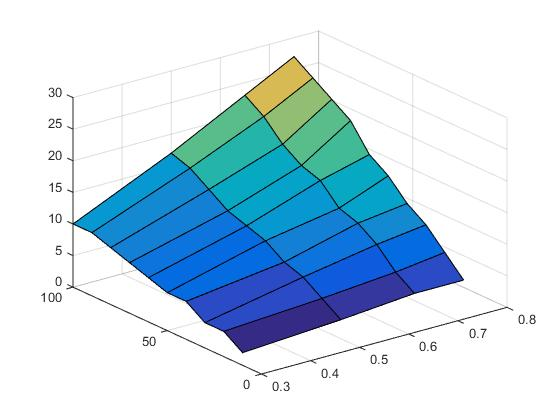
\includegraphics[width=8cm]{MinColor}
\centering
\caption{$Z$ is the minimum number of colors needed. $X-Y$ plane is $density-number of vertices$ }
\label{fig:mincolor}
\end{figure}

Further analysis reveal the relation among number of minimum colors $y$ , density $d$ and number of nodes $|V|$. Data points of the same density are fitted into a line and $R^{2}$ are calculated. Figure \ref{fig:coloranalysis} has more details. Equations are shown in the figure.

\begin{figure}[htp]
\centering
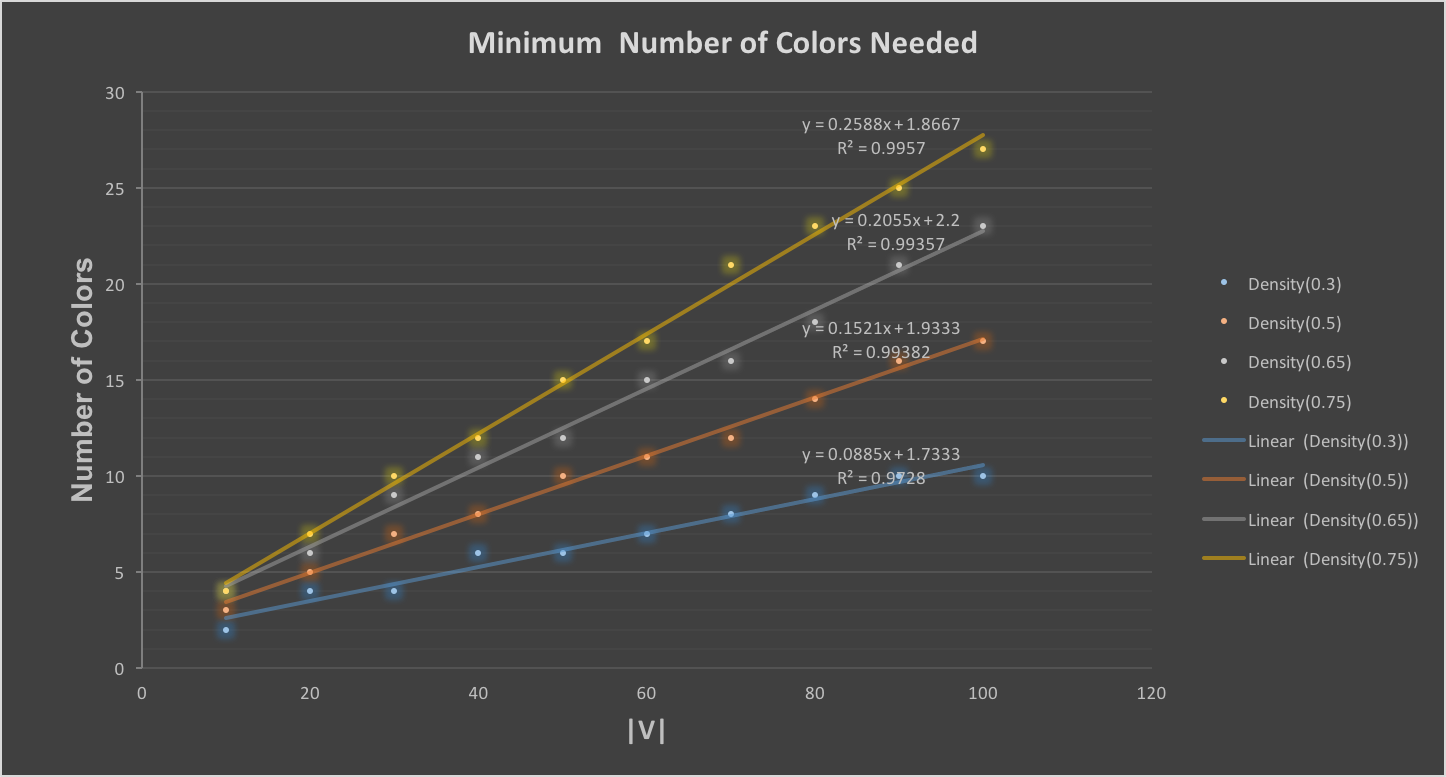
\includegraphics[width=13cm]{minimumcolor}
\centering
\caption{Apply linear regression. $y = f(|V|)$ }
\label{fig:coloranalysis}
\end{figure}

The $R^{2}$ shows a strong linear relation between $y$ and $|V|$. It is also reasonable to speculate that the intercept should be 2 since any bipartite graph with any number of vertices only need two colors. But more serious thoughts and proof are required to explore this relationship.
What's more, it is very interesting to see the slopes in the Figure \ref{fig:coloranalysis} are also a function of density. Data in table \ref{tab:slope-density} is used to apply linear regression. Table \ref{tab:density-slope} shows the result. The adjusted $R^{2}$ is very close to 1.

\begin{table}[H]
    \centering
    \begin{tabular}{ccc}
    \toprule
        Density & Square of Density & Slope\\
       \midrule
        0.3 & 0.09 &  0.0885\\
        0.5 & 0.25 & 0.1521 \\
        0.65& 0.4225 &0.2055 \\
       0.75 & 0.5625 & 0.2588 \\
      \bottomrule
    \end{tabular}
    \caption{Density - Slope Data}
    \label{tab:slope-density}
\end{table}

\begin{table}[H]
    \centering
    \begin{tabular}{llll}
    \toprule
        Indicators & Value &  & Coefficients\\
       \midrule
        $R^{2}$ & 0.9982 & Intercept &0.04235 \\
        Adjusted $R^{2}$ & 0.9947 & Density Square & 0.28894\\
        Standard Error & 0.005308 & Density & 0.06939\\
      \bottomrule
    \end{tabular}
    \caption{Density - Slope Regression Statistics}
    \label{tab:density-slope}
\end{table}

The conclusion is that the minimum number of colors needed to color a random graph $y$ is a function of density  $d$ and number of nodes $|V|$ in this form: \\
$y = (0.289d^{2}+0.0691d+0.042)|V|+2$.

\section{Experiment Results}\label{sec:data}

\newpage
\subsection{Runningt Time Statistics}
Average running time per graph in milliseconds and statistics about density.

\begin{table}[H]
    \centering
    \begin{tabular}{ccclll}
    \toprule
$|V|$ & running time($10^{-3}$s) & Target Density & Avg Density & Max Density & Min Density\\ 
       \midrule
10 & 0.09 & 0.3 & 0.301555556 & 0.377777778 & 0.244444444\\ 
20 & 0.07 & 0.3 & 0.298421053 & 0.331578947 & 0.3\\ 
30 & 0.1 & 0.3 & 0.296413793 & 0.324137931 & 0.294252874\\ 
40 & 1.6 & 0.3 & 0.300538462 & 0.317948718 & 0.28974359\\ 
50 & 0.2 & 0.3 & 0.299395918 & 0.333877551 & 0.293061224\\ 
60 & 0.26 & 0.3 & 0.30200565 & 0.307909605 & 0.298870056\\ 
70 & 0.41 & 0.3 & 0.299337474 & 0.300621118 & 0.289855072\\ 
80 & 0.38 & 0.3 & 0.300047468 & 0.310759494 & 0.292721519\\ 
90 & 0.44 & 0.3 & 0.299558052 & 0.303620474 & 0.296878901\\ 
100 & 0.25 & 0.3 & 0.29879596 & 0.300606061 & 0.291919192\\ 
      \bottomrule
    \end{tabular}
    \caption{Running Time Statistics (density=0.3)}
    \label{tab:running time (density=0.3)}
\end{table}

\begin{table}[H]
    \centering
    \begin{tabular}{ccclll}
    \toprule
$|V|$ & running time($10^{-3}$s) & Target Density & Avg Density & Max Density & Min Density\\ 
       \midrule
10 & 0.14 & 0.5 & 0.501777778 & 0.555555556 & 0.422222222\\ 
20 & 0.09 & 0.5 & 0.504473684 & 0.552631579 & 0.473684211\\ 
30 & 0.15 & 0.5 & 0.502068966 & 0.505747126 & 0.498850575\\ 
40 & 0.2 & 0.5 & 0.500948718 & 0.508974359 & 0.483333333\\ 
50 & 0.25 & 0.5 & 0.500636735 & 0.515918367 & 0.489795918\\ 
60 & 0.28 & 0.5 & 0.499734463 & 0.501129944 & 0.476836158\\ 
70 & 0.37 & 0.5 & 0.501031056 & 0.506832298 & 0.479917184\\ 
80 & 0.37 & 0.5 & 0.499006329 & 0.509493671 & 0.499367089\\ 
90 & 0.46 & 0.5 & 0.499662921 & 0.502871411 & 0.487141074\\ 
100 & 0.38 & 0.5 & 0.4998 & 0.502020202 & 0.495555556\\ 
      \bottomrule
    \end{tabular}
    \caption{Running Time Statistics (density=0.5)}
    \label{tab:running time (density=0.5)}
\end{table}

\begin{table}[H]
    \centering
    \begin{tabular}{ccclll}
    \toprule
$|V|$ & running time($10^{-3}$s) & Target Density & Avg Density & Max Density & Min Density\\ 
       \midrule
10 & 0.11 & 0.65 & 0.648888889 & 0.666666667 & 0.622222222\\ 
20 & 0.1 & 0.65 & 0.656578947 & 0.726315789 & 0.642105263\\ 
30 & 0.2 & 0.65 & 0.651264368 & 0.67816092 & 0.625287356\\ 
40 & 0.28 & 0.65 & 0.646448718 & 0.655128205 & 0.629487179\\ 
50 & 0.43 & 0.65 & 0.648971429 & 0.669387755 & 0.647346939\\ 
60 & 0.44 & 0.65 & 0.649870056 & 0.651977401 & 0.648587571\\ 
70 & 0.54 & 0.65 & 0.649300207 & 0.661697723 & 0.649689441\\ 
80 & 0.42 & 0.65 & 0.649860759 & 0.652848101 & 0.635443038\\ 
90 & 0.74 & 0.65 & 0.648836454 & 0.657677903 & 0.649188514\\ 
100 & 5.1 & 0.65 & 0.649878788 & 0.65010101 & 0.648888889\\ 
      \bottomrule
    \end{tabular}
    \caption{Running Time Statistics (density=0.65)}
    \label{tab:running time (density=0.65)}
\end{table}

\begin{table}[H]
    \centering
    \begin{tabular}{ccclll}
    \toprule
$|V|$ & running time($10^{-3}$s) & Target Density & Avg Density & Max Density & Min Density\\ 
       \midrule
10 & 0.13 & 0.75 & 0.75 & 0.8 & 0.733333333\\ 
20 & 0.1 & 0.75 & 0.749210526 & 0.752631579 & 0.715789474\\ 
30 & 0.23 & 0.75 & 0.747310345 & 0.751724138 & 0.744827586\\ 
40 & 0.3 & 0.75 & 0.748166667 & 0.752564103 & 0.734615385\\ 
50 & 0.51 & 0.75 & 0.748669388 & 0.76244898 & 0.737142857\\ 
60 & 0.49 & 0.75 & 0.749971751 & 0.755367232 & 0.744632768\\ 
70 & 0.55 & 0.75 & 0.749925466 & 0.754865424 & 0.744513458\\ 
80 & 0.51 & 0.75 & 0.749987342 & 0.75221519 & 0.728797468\\ 
90 & 0.46 & 0.75 & 0.749702871 & 0.75855181 & 0.734332085\\ 
100 & 2.63 & 0.75 & 0.750179798 & 0.756363636 & 0.743232323\\ 
      \bottomrule
    \end{tabular}
    \caption{Running Time Statistics (density=0.75)}
    \label{tab:running time (density=0.75)}
\end{table}

\newpage
\subsection{Color Statistics}
Statistics about number of colors.

\begin{table}[H]
    \centering
    \begin{tabular}{cclllll}
    \toprule
$|V|$ & Target Density & Avg \#colors & Max \#colors &  Min \#colors & Std \#colors & Median\#colors\\ 
       \midrule
10 & 0.3 & 3.02 & 4 & 2 & 0.42592739 & 3\\ 
20 & 0.3 & 4.32 & 5 & 4 & 0.468826172 & 4\\ 
30 & 0.3 & 5.31 & 7 & 4 & 0.525991128 & 5\\ 
40 & 0.3 & 6.43 & 7 & 6 & 0.497569852 & 6\\ 
50 & 0.3 & 7.31 & 8 & 6 & 0.525991128 & 7\\ 
60 & 0.3 & 8.24 & 9 & 7 & 0.49482167 & 8\\ 
70 & 0.3 & 9.18 & 10 & 8 & 0.47947783 & 9\\ 
80 & 0.3 & 10.04 & 11 & 9 & 0.530294372 & 10\\ 
90 & 0.3 & 10.87 & 12 & 10 & 0.485236587 & 11\\ 
100 & 0.3 & 11.68 & 13 & 10 & 0.583960702 & 12\\ 
      \bottomrule
    \end{tabular}
    \caption{Color Statistics (density=0.3)}
    \label{tab:colors(density=0.3)}
\end{table}

\begin{table}[H]
    \centering
    \begin{tabular}{cclllll}
    \toprule
$|V|$ & Target Density & Avg \#colors & Max \#colors &  Min \#colors & Std \#colors & Median\#colors\\ 
       \midrule
10 & 0.5 & 4 & 5 & 3 & 0.53182 & 4\\ 
20 & 0.5 & 6.08 & 8 & 5 & 0.58049 & 6\\ 
30 & 0.5 & 7.85 & 9 & 7 & 0.64157 & 8\\ 
40 & 0.5 & 9.45 & 11 & 8 & 0.60927 & 9\\ 
50 & 0.5 & 11.07 & 12 & 10 & 0.65528 & 11\\ 
60 & 0.5 & 12.6 & 15 & 11 & 0.71067 & 13\\ 
70 & 0.5 & 14.1 & 16 & 12 & 0.70353 & 14\\ 
80 & 0.5 & 15.7 & 17 & 14 & 0.70353 & 16\\ 
90 & 0.5 & 16.97 & 18 & 16 & 0.68836 & 17\\ 
100 & 0.5 & 18.32 & 20 & 17 & 0.77694 & 18\\ 
      \bottomrule
    \end{tabular}
    \caption{Color Statistics (density=0.5)}
    \label{tab:colors(density=0.5)}
\end{table}

\begin{table}[H]
    \centering
    \begin{tabular}{cclllll}
    \toprule
$|V|$ & Target Density & Avg \#colors & Max \#colors &  Min \#colors & Std \#colors & Median\#colors\\ 
       \midrule
10 & 0.65 & 4.83 & 6 & 4 & 0.62044 & 5\\ 
20 & 0.65 & 7.68 & 9 & 6 & 0.61759 & 8\\ 
30 & 0.65 & 10.14 & 12 & 9 & 0.84112 & 10\\ 
40 & 0.65 & 12.25 & 14 & 11 & 0.83333 & 12\\ 
50 & 0.65 & 14.31 & 16 & 12 & 0.82505 & 14\\ 
60 & 0.65 & 16.59 & 19 & 15 & 0.76667 & 17\\ 
70 & 0.65 & 18.6 & 21 & 16 & 0.98473 & 19\\ 
80 & 0.65 & 20.7 & 23 & 18 & 0.87039 & 21\\ 
90 & 0.65 & 22.59 & 25 & 21 & 0.93306 & 23\\ 
100 & 0.65 & 24.52 & 27 & 23 & 0.88169 & 25\\
      \bottomrule
    \end{tabular}
    \caption{Color Statistics (density=0.65)}
    \label{tab:colors(density=0.65)}
\end{table}

\begin{table}[H]
    \centering
    \begin{tabular}{cclllll}
    \toprule
$|V|$ & Target Density & Avg \#colors & Max \#colors &  Min \#colors & Std \#colors & Median\#colors\\ 
       \midrule
10 & 0.75 & 5.65 & 9 & 4 & 0.85723 & 6\\ 
20 & 0.75 & 8.89 & 11 & 7 & 0.72328 & 9\\ 
30 & 0.75 & 11.82 & 14 & 10 & 0.80879 & 12\\ 
40 & 0.75 & 14.69 & 17 & 12 & 0.89550 & 15\\ 
50 & 0.75 & 17.37 & 19 & 15 & 0.86053 & 17\\ 
60 & 0.75 & 19.9 & 22 & 17 & 0.98985 & 20\\ 
70 & 0.75 & 22.38 & 25 & 21 & 1.08971 & 22\\ 
80 & 0.75 & 25.07 & 27 & 23 & 1.02745 & 25\\ 
90 & 0.75 & 27.27 & 30 & 25 & 1.09041 & 27\\ 
100 & 0.75 & 29.58 & 32 & 27 & 1.00685 & 30\\
      \bottomrule
    \end{tabular}
    \caption{Color Statistics (density=0.75)}
    \label{tab:colors(density=0.75)}
\end{table}

\section{Acknowledgement}
This assignment is done by Jiacheng Liu alone. 

\begin{thebibliography}{10}
\bibitem{DSatur} 
Brélaz, Daniel. 
"New methods to color the vertices of a graph." 
\textit{Communications of the ACM} 22.4 (1979): 251-256.

\end{thebibliography}

\end{document}
